\section{Kinematic Modeling and Planning Formulation}
This section defines the vehicle geometry and stopping rule, derives the discrete cable closure, and combines it with collision constraints and the planning objective.

\begin{figure*}[!t]
\centering
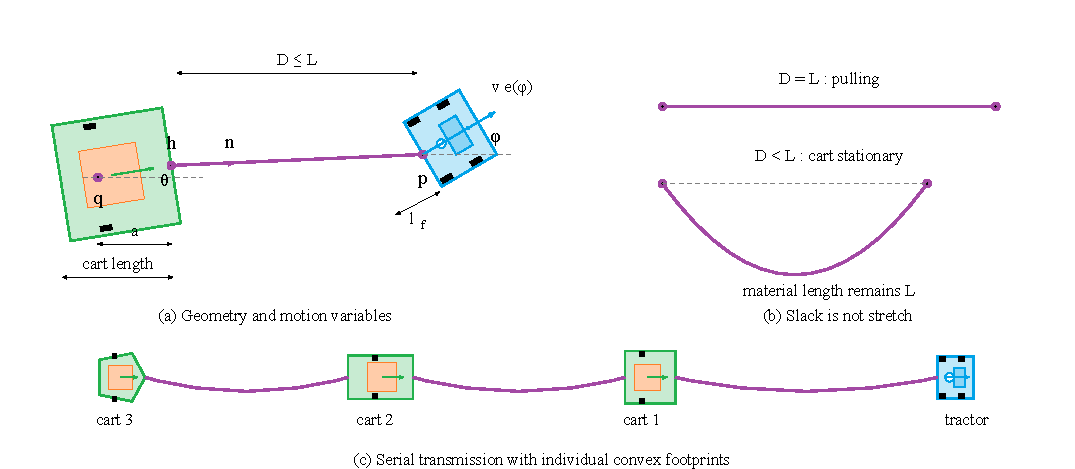
\includegraphics[width=\textwidth]{kinematics.pdf}
\caption{Vehicle geometry, slack--taut cable states, and serial transmission to passive carts.}
\label{fig:kinematics}
\end{figure*}
\subsection{Geometry and Operating Assumptions}
Let $\pp\in\mathbb R^2$ and $\phi$ denote the tractor rear-axle position and heading. The cable attaches at $\pp$ and at the cart hitch $\hh\in\mathbb R^2$. The cart heading is $\theta$, the hitch-to-axle offset is $a>0$, and $\ee(\alpha)=(\cos\alpha,\sin\alpha)^\top$. Its axle position is the algebraic output
\begin{equation}
\qq=\hh-a\ee(\theta).
\label{eq:axle}
\end{equation}
Define $\ee_\perp(\alpha)=[-\sin\alpha,\cos\alpha]^\top$ and
\begin{equation}
\begin{aligned}
D&=\|\pp-\hh\|_2,\\
\nn&=(\pp-\hh)/D,\\
D&>0,\\
D&\leq L.
\end{aligned}
\label{eq:cable}
\end{equation}
The cable material length $L$ is constant. The inequality $D<L$ describes slack accommodated by cable bending. The independent state is $\xx=(p_x,p_y,\phi,h_x,h_y,\theta)$.

The tractor follows bicycle kinematics with signed speed $v$, wheelbase $\ell_f$, steering angle $\delta$, and curvature $\kappa=\tan\delta/\ell_f$. The cart is assumed to stop immediately when no pulling motion is transmitted. In the pulling regime, a nominal hitch-mobility closure specifies that its hitch moves along the cable direction. With pulling speed $w\geq0$,
\begin{equation}\begin{aligned}
\dot\pp&=v\ee(\phi),\\
\dot\phi&=v\kappa,\\
\dot\hh&=w\nn,\\
\dot\theta&=\frac{w}{a}\nn^\top\ee_\perp(\theta).
\end{aligned}\label{eq:continuous}\end{equation}
This explicit first-order hitch-mobility closure specifies the pulling response. It implies
\begin{equation}
\dot\qq=w\bigl(\nn^\top\ee(\theta)\bigr)\ee(\theta),
\label{eq:nonholonomic}
\end{equation}
so the continuous axle velocity has no lateral component. The nonreversing cart rule is $w\nn^\top\ee(\theta)\geq0$. The tractor's $v$ can have either sign.

For $D<L$, the instantaneous unpulled state has $w=0$. On the taut boundary, outward tractor motion gives $w=\max\{0,\nn^\top\dot\pp\}$. Motion directed inward creates slack and stops the cart. The operating premise is quasistatic low-speed transport with sufficiently rapid stopping when pulling ceases. This first-order abstraction specifies the nominal motion used for planning; physical applicability depends on the stopping and hitch-mobility behavior of the cart.

\subsection{Euler Updates With an Inextensible Endpoint Closure}
For an interval of duration $\Delta t_k$, write $s_k=v_k\Delta t_k$ and $W_k=w_k\Delta t_k$. The optimization parameterizes motion by displacement increments and curvature. All independent states use first-order explicit Euler updates:
\begin{equation}\begin{aligned}
\pp_{k+1}&=\pp_k+s_k\ee(\phi_k),\\
\phi_{k+1}&=\phi_k+s_k\kappa_k,\\
\hh_{k+1}&=\hh_k+W_k\nn_k,\\
\theta_{k+1}&=\theta_k+\frac{W_k}{a}\nn_k^\top\ee_\perp(\theta_k).
\end{aligned}\label{eq:euler}\end{equation}
The axle position is evaluated algebraically from~\eqref{eq:axle} at every node.

The end-of-step cable condition closes $W_k$ algebraically. Set $c_k=\nn_k^\top\ee(\phi_k)$. From~\eqref{eq:euler},
\begin{equation}
\|\pp_{k+1}-\hh_{k+1}\|_2^2
=(D_k+s_kc_k-W_k)^2+s_k^2(1-c_k^2).
\label{eq:quadratic}
\end{equation}
Define the unconstrained closure displacement
\begin{equation}
\eta_k=D_k+s_kc_k-\sqrt{L^2-s_k^2(1-c_k^2)}.
\label{eq:eta}
\end{equation}
Then the common discrete mode relation is
\begin{equation}
W_k=\max\{0,\eta_k\}.
\label{eq:max}
\end{equation}

\begin{proposition}[Discrete unilateral closure]
Suppose $0<|s_k|<D_k\leq L$. Equation~\eqref{eq:max} is the minimum nonnegative hitch displacement along $\nn_k$ that satisfies the endpoint length bound. If the free endpoint remains within distance $L$ of the stationary hitch, $W_k=0$. Otherwise, the endpoint distance equals $L$ after the update. Moreover, $-L<\eta_k\leq |s_k|$.
\label{prop:closure}
\end{proposition}
\begin{IEEEproof}
The radicand in~\eqref{eq:eta} is positive. Since $D_k+s_kc_k>D_k-|s_k|>0$, the two roots of~\eqref{eq:quadratic} at squared distance $L^2$ delimit the feasible hitch-displacement interval. Its smaller endpoint is $\eta_k$, and its larger endpoint is positive. Intersecting this interval with $W_k\geq0$ gives the minimum $\max\{0,\eta_k\}$. Also, $D_k+s_kc_k>0$ and the square root is at most $L$, yielding $\eta_k>-L$. Let $r=|s_k|$ and $u=s_kc_k/r$. The function $ru-\sqrt{L^2-r^2+r^2u^2}$ increases on $[-1,1]$, since $\sqrt{L^2-r^2+r^2u^2}>|ru|$. Thus $\eta_k\leq D_k+r-L\leq r$.
\end{IEEEproof}

For $s_k=0$, the relation gives $W_k=0$ directly. The closure is exact for the stated discrete Euler model. Consequently,~\eqref{eq:euler}--\eqref{eq:max} preserve the endpoint bound in exact arithmetic and stop both hitch translation and cart rotation on an entirely slack step. A step crossing from slack to taut represents an average pulling increment over the integration interval. On the taut boundary, the first-order limit is $W_k/\Delta t_k\to\max\{0,\nn_k^\top\dot\pp_k\}$. The algebraic axle output has an $O(W_k^2)$ lateral displacement relative to its current heading, consistent with first-order state integration. Every compared method uses this Euler transcription with algebraic endpoint closure.

\subsection{Equivalent Exact Mode Representations}
Let $s_{\max}$ bound the signed tractor increment and let $D_{\min}$ bound the endpoint distance from below, with $0<s_{\max}<D_{\min}\leq L$. For fixed values of the geometric expression $\eta_k$, the graph of~\eqref{eq:max} has the exact complementarity representation
\begin{equation}
\begin{aligned}
 &W_k\geq0,\\
 &W_k-\eta_k\geq0,\\
 &W_k(W_k-\eta_k)=0.
\end{aligned}
\label{eq:comp}
\end{equation}
It also admits a binary representation with $z_k\in\{0,1\}$:
\begin{equation}\begin{aligned}
 &W_k\geq0,\\
 &W_k\geq\eta_k,\\
 &W_k\leq s_{\max}z_k,\\
 &W_k\leq\eta_k+L(1-z_k).
\end{aligned}\label{eq:minlp}\end{equation}
Proposition~\ref{prop:closure} establishes the sufficient constants $s_{\max}$ and $L$; an arbitrary large constant is unnecessary. For $z_k=0$,~\eqref{eq:minlp} forces $W_k=0$ and $\eta_k\leq0$. For $z_k=1$, it forces $W_k=\eta_k\geq0$. Conversely, either branch of~\eqref{eq:max} satisfies~\eqref{eq:minlp}. At $\eta_k=0$, either binary label describes the same state update. A conditional expression selecting $\eta_k$ when $\eta_k\geq0$ and zero otherwise is another implementation of the same graph. Fixing $z_k$ from an initial trajectory restricts this graph to the chosen mode sequence.

These equivalences concern the declared discrete model. They permit a controlled comparison of expression and solution strategies without changing the physical assumptions or discretization.

\subsection{Body Geometry, Collision Constraints, and Cable Routing}
Each body has a convex polygonal footprint of arbitrary shape. The local halfspace matrix and vector are computed from its actual vertices; no rectangular replacement is used. In local coordinates, let $\mathcal B=\{y:Gy\leq g\}$. Its world footprint is $\mathcal E_k=\RR(\alpha_k)\mathcal B+t_k$, where $\RR(\alpha)$ is the planar rotation matrix and $(t_k,\alpha_k)$ equals $(\pp_k,\phi_k)$ or $(\qq_k,\theta_k)$. For a convex obstacle $\mathcal O=\{y:Ay\leq b\}$, the OBCA distance certificate~\cite{obca2021} introduces $\lambda_k,\mu_k\geq0$ for a prescribed planning clearance $d_{\rm plan}>0$, satisfying
\begin{equation}\begin{aligned}
 &G^\top\mu_k+\RR(\alpha_k)^\top A^\top\lambda_k=0,\\
 &\|A^\top\lambda_k\|_2\leq1,\\
 &(At_k-b)^\top\lambda_k-g^\top\mu_k\geq d_{\rm plan}.
\end{aligned}\label{eq:obca}\end{equation}
The same dual construction is imposed between the two vehicle bodies and against workspace walls. Independent polygon-distance evaluation subsequently checks the primal trajectory rather than relying on the dual variables or solver status alone.

Cable collision is treated separately from body separation. For $D<L$, the routing audit constructs the smooth planar curve
\begin{equation}
\mathbf r(t)=\hh+t(\pp-\hh)+4\alpha t(1-t)\nn_\perp,
\label{eq:route}
\end{equation}
for $t\in[0,1]$, where $\nn_\perp=(-n_y,n_x)^\top$ and the lateral bow amplitude $\alpha\geq0$ is selected so that the analytic arc length equals $L$. Its arc length is
\begin{equation}
\mathcal L(\alpha)=\tfrac12\sqrt{D^2+16\alpha^2}
+\frac{D^2}{8\alpha}\operatorname{asinh}(4\alpha/D).
\label{eq:arclength}
\end{equation}
The continuous limit at zero amplitude is $D$. Either lateral orientation may be checked; a taut cable is a straight segment. In the most compact mechanism cases, a symmetric curve can enter a vehicle near an attachment. The audit then also tests the smooth asymmetric family obtained by replacing $4t(1-t)$ with $f_\beta(t)=4t(1-t)[1+\beta(2t-1)]$. Its amplitude is selected from $\int_0^1\sqrt{D^2+\alpha^2[f_\beta' (t)]^2}\,dt=L$, checked by independent numerical quadrature. This routing freedom changes neither endpoint kinematics nor material length. The warehouse solver comparisons use the same symmetric routing filter throughout; asymmetric routes are an additional geometric witness for the compact mechanism suite. A segmented evaluation of the curve tests walls, obstacles, and body interiors, with the quadratic chord-error bound applied to obstacle checks. An accepted curve is a per-node geometric routing witness: it establishes the existence of a collision-free cable route of the prescribed length at that configuration. Continuous shape evolution and snag-free execution require a physical cable-interaction model. All methods use this same routing filter.

\subsection{Serial Cable-Towed Carts}
For cart $i$, let $\hh_i$ be its front hitch, $\theta_i$ its heading, $a_i$ its hitch-to-axle distance, and $b_i$ the distance from the axle to the rear attachment. Its rear attachment is $\mathbf t_i=\hh_i-(a_i+b_i)\ee(\theta_i)$. Cable $i$ connects $\hh_i$ to $\mathbf t_{i-1}$, with $\mathbf t_0=\pp$. Define the material length $L_i$, endpoint distance $D_i=\|\mathbf t_{i-1}-\hh_i\|_2$, and direction $\nn_i=(\mathbf t_{i-1}-\hh_i)/D_i$. Once the upstream attachment displacement $\Delta\mathbf t_{i-1}$ is known, the same endpoint closure gives
\begin{equation}\begin{aligned}
c_i&=\nn_i^\top\Delta\mathbf t_{i-1},\\
W_i&=\max\!\left\{0,D_i+c_i-\sqrt{L_i^2-\|\Delta\mathbf t_{i-1}\|^2+c_i^2}\right\}.
\end{aligned}\label{eq:serial}\end{equation}
The hitch and heading use the Euler updates in~\eqref{eq:euler} with indices $i$. Propagation proceeds from the tractor toward the final cart. A stationary upstream attachment produces zero downstream displacement, consistent with the stop-on-slack rule. Positive radicands and step bounds are required at every link. The OBCA construction extends to all body pairs and all body--obstacle pairs, using each cart's own footprint.

\subsection{Optimization Problem}
For a common grid of $N$ intervals, the decision variables are the states, $(s_k,\kappa_k,W_k)$, and OBCA dual variables, with binary variables only in~\eqref{eq:minlp}. The objective is
\begin{equation}
\begin{aligned}
J&=\sum_{k=0}^{N-1}\ell_k+\gamma\sum_{k=1}^{N-1}(\kappa_k-\kappa_{k-1})^2,\\
\ell_k&\geq s_k,\\
\ell_k&\geq -s_k.
\end{aligned}
\label{eq:cost}
\end{equation}
The first term measures tractor travel; the second discourages abrupt changes in the curvature sequence. The nonnegative travel epigraph $\ell_k$ equals $\max\{s_k,-s_k\}$ at a minimum. Reported costs are recomputed from the actual controls with this exact travel value. The same weight $\gamma$ is used by every method, with its numerical value listed in the experimental settings.

The constraints are the prescribed initial state,~\eqref{eq:euler}, one exact mode representation,~\eqref{eq:obca}, the terminal transport task, and
\begin{equation}\begin{aligned}
 &s_k\geq-s_{\max},\\
 &s_k\leq s_{\max},\\
 &\kappa_k\geq-R_{\min}^{-1},\\
 &\kappa_k\leq R_{\min}^{-1},\\
 &D_k\geq D_{\min},\\
 &D_k\leq L,\\
 &W_k\nn_k^\top\ee(\theta_k)\geq0.
\end{aligned}\label{eq:bounds}\end{equation}
The stated relation among $s_{\max}$, $D_{\min}$, and $L$ satisfies Proposition~\ref{prop:closure}. The terminal task specifies a rear-axle goal region and desired tractor and cart headings. This permits side loading, turns, and return routes. The numerical implementation bounds headings in $[-\pi,\pi]$ and positions within the workspace; task headings are represented continuously within that interval. All methods use identical state and terminal bounds for each case. Numerical dimensions, tolerances, and solver settings are collected in Section~V.

\subsection{A Reachability Separation From Rigid Coupling}
Consider a conventional rigid-drawbar system with the same vehicle bodies and drawbar length $L$. Its hitch relation is
\begin{equation}
\pp=\qq+(a+L)\ee(\theta).
\label{eq:rigid}
\end{equation}
The tongue is fixed relative to the cart and pivots at the tractor attachment. Both vehicles may move forward or backward. This comparator has the same fully extended longitudinal span as the initially taut cable system.

For this comparison, both footprints are rectangles. Let $b_r$ be the cart rear overhang, $c_f$ the tractor's forward extent, and $w_r,w_f$ the respective half-widths. Define $A_0=a+L+b_r$. The vehicles start aligned with the horizontal direction inside an infinite vertical strip. After subtracting wall clearances, the available horizontal width is $A_0+c_f+\epsilon$.

\begin{theorem}[Rigid strip barrier]
If
\begin{equation}
\begin{aligned}
 &\epsilon>0,\\
 &\epsilon<B_*,\\
 &B_*=\min\{B_\theta,B_\phi\},\\
 &B_\theta=\sqrt{A_0^2+w_r^2}-A_0,\\
 &B_\phi=\sqrt{c_f^2+w_f^2}-c_f.
\end{aligned}
\label{eq:barrier}
\end{equation}
no continuous collision-free configuration path satisfying~\eqref{eq:rigid} can reorient the initially aligned combination to cart heading $\pi/2$, regardless of the sequence of forward and backward controls.
\label{thm:rigid}
\end{theorem}
\begin{IEEEproof}
Define the limiting cart and tractor headings by $\theta_*=\arctan(w_r/A_0)$ and $\phi_*=\arctan(w_f/c_f)$, respectively. Within the angle box $|\theta|\leq\theta_*$, $|\phi|\leq\phi_*$, the horizontal distance from the cart's leftmost corner to the tractor's rightmost corner is
\begin{equation}
H=A_0\cos\theta+w_r|\sin\theta|
+c_f\cos\phi+w_f|\sin\phi|.
\label{eq:span}
\end{equation}
It is a lower bound on the occupied width, independent of translation. Each of the two angle-dependent terms is at least its initial value, $A_0$ or $c_f$, within this box. Any continuous path from zero headings to the target must first reach the box boundary. There, at least one term reaches its maximum, either $\sqrt{A_0^2+w_r^2}$ or $\sqrt{c_f^2+w_f^2}$. Thus $H\geq A_0+c_f+B_*>A_0+c_f+\epsilon$, contradicting the available width. The proof imposes no restriction on control direction.
\end{IEEEproof}

Cable coupling allows the taut cable direction to differ from the cart heading. Slack further permits the tractor to reverse and rotate while the cart waits, then pull it into the vertical transport direction. Section~V constructs numerical trajectories for a parameterized family satisfying~\eqref{eq:barrier}. Theorem~\ref{thm:rigid} certifies the rigid system's continuous geometric obstruction, while independent Euler replay and per-node cable-route checks establish feasibility of the cable maneuvers under the prescribed discrete model.